\section{System Design} In this section, we describe the flow diagram of the application given in Figure \ref{fig:design}. For the application, we have developed the following React components.
\begin{figure}[htp]
	\centering
	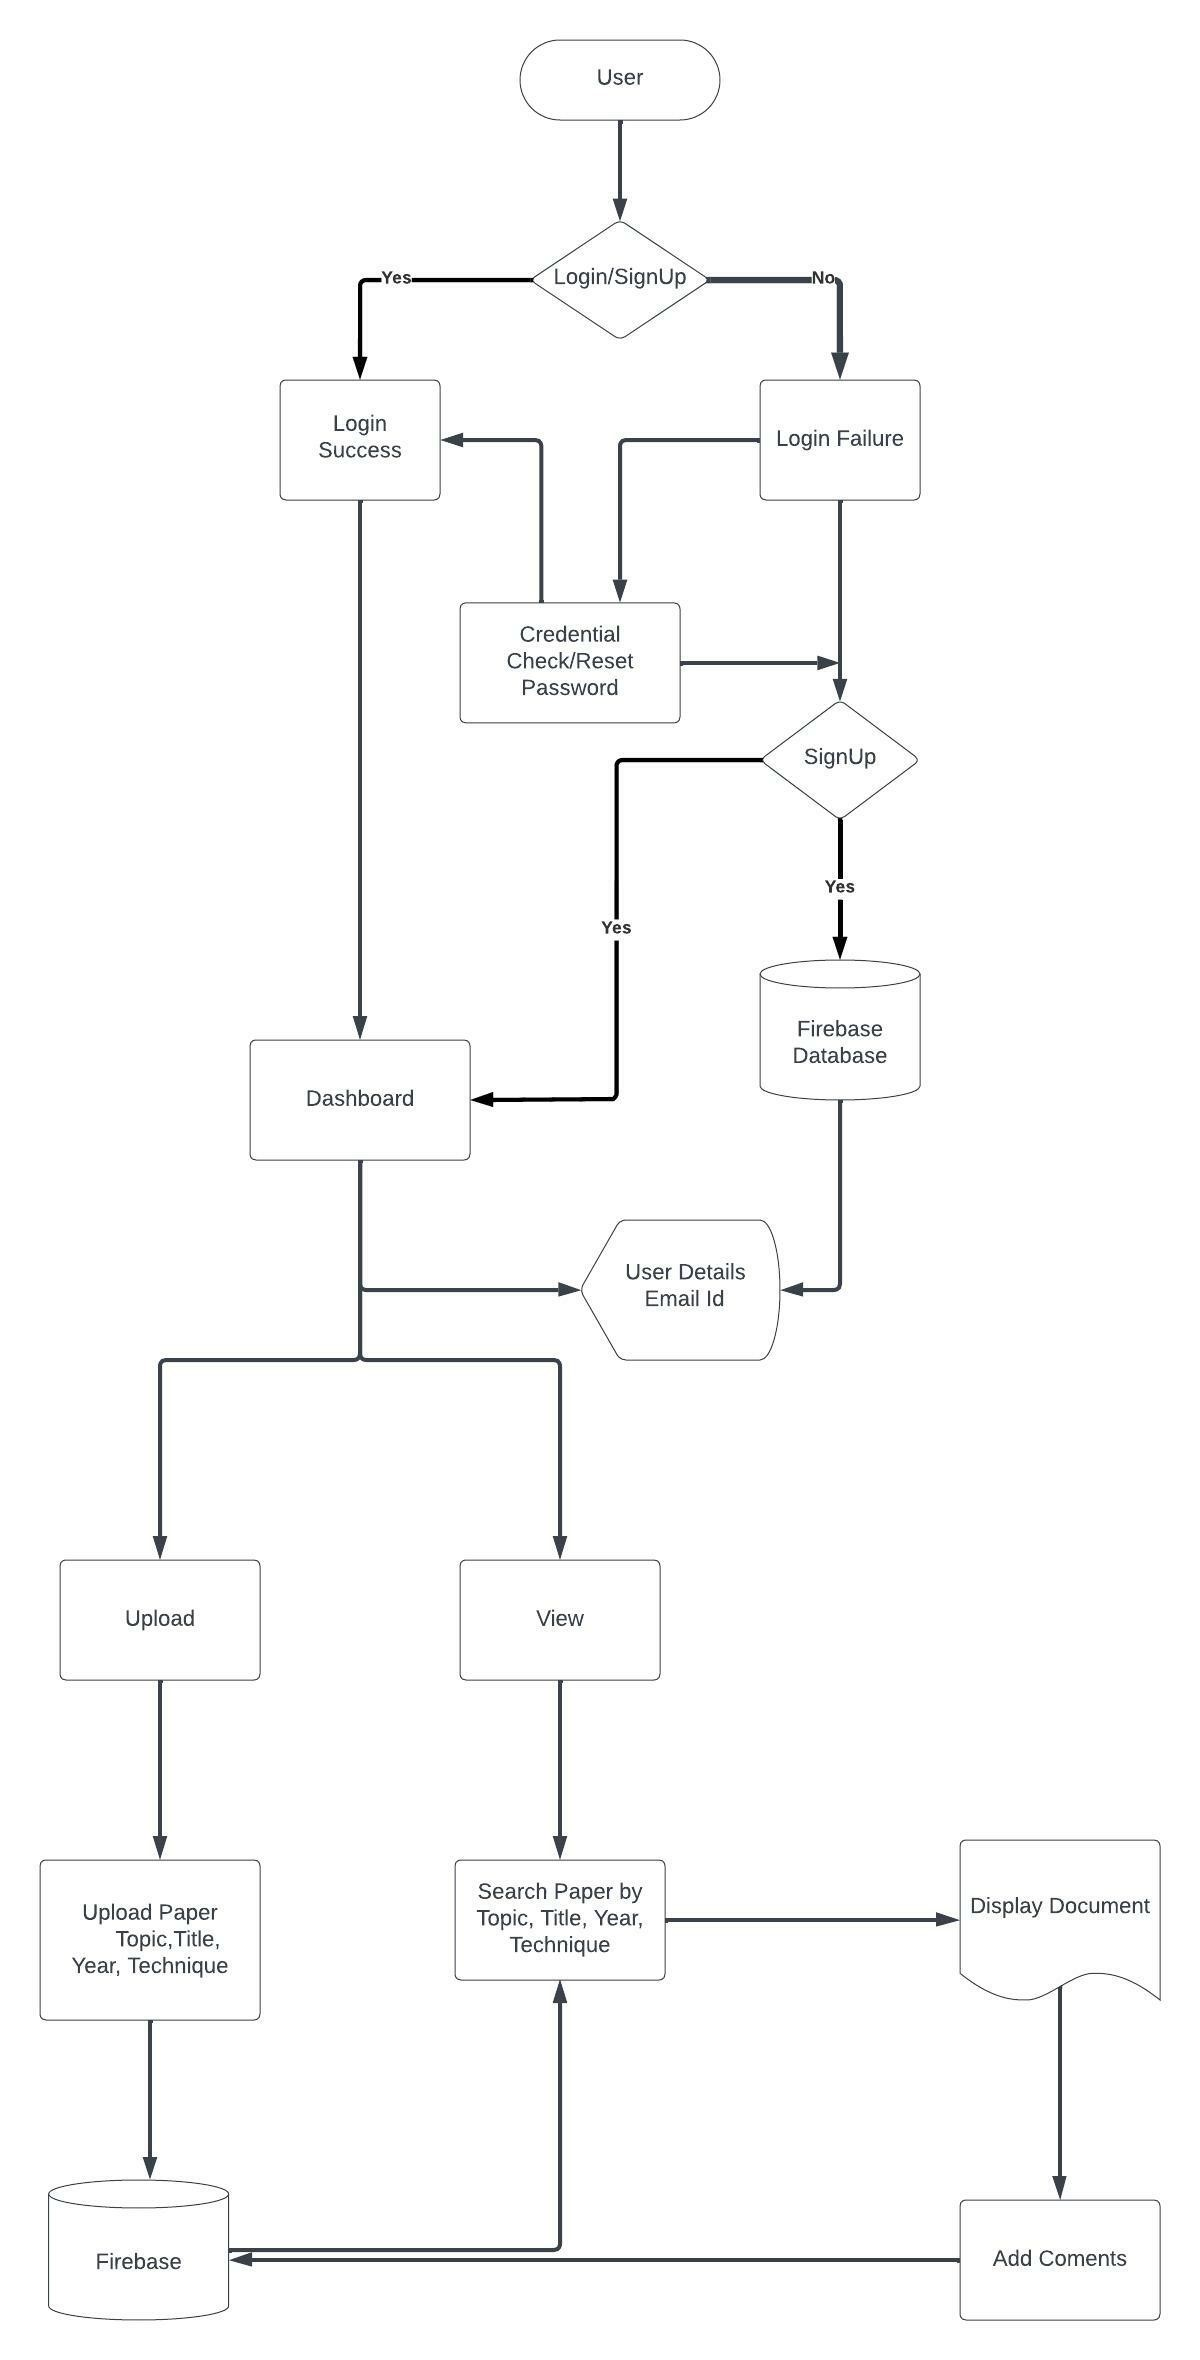
\includegraphics[width=11cm,height=12.5cm]{./images/flow.jpg}
	\caption{Research Content Management}
	\label{fig:design}
\end{figure}
\paragraph{\textbf{Register:}} For the new users, we 
have developed a register component for creating an account on the application shown in Figure \ref{fig:register}. To register, the users have to fill up their information, namely, name, email, and password. 

We also provide another option to users for registering through their google account, that is, if one has a valid Google account saved in his local machine, he/she can register at a glance using the above mentioned feature. The authentication requirements provided by the Firebase are needed to meet like password should be minimum of 6 characters in length and email address should end up with .com. 
\begin{figure}[t]
	\centering
	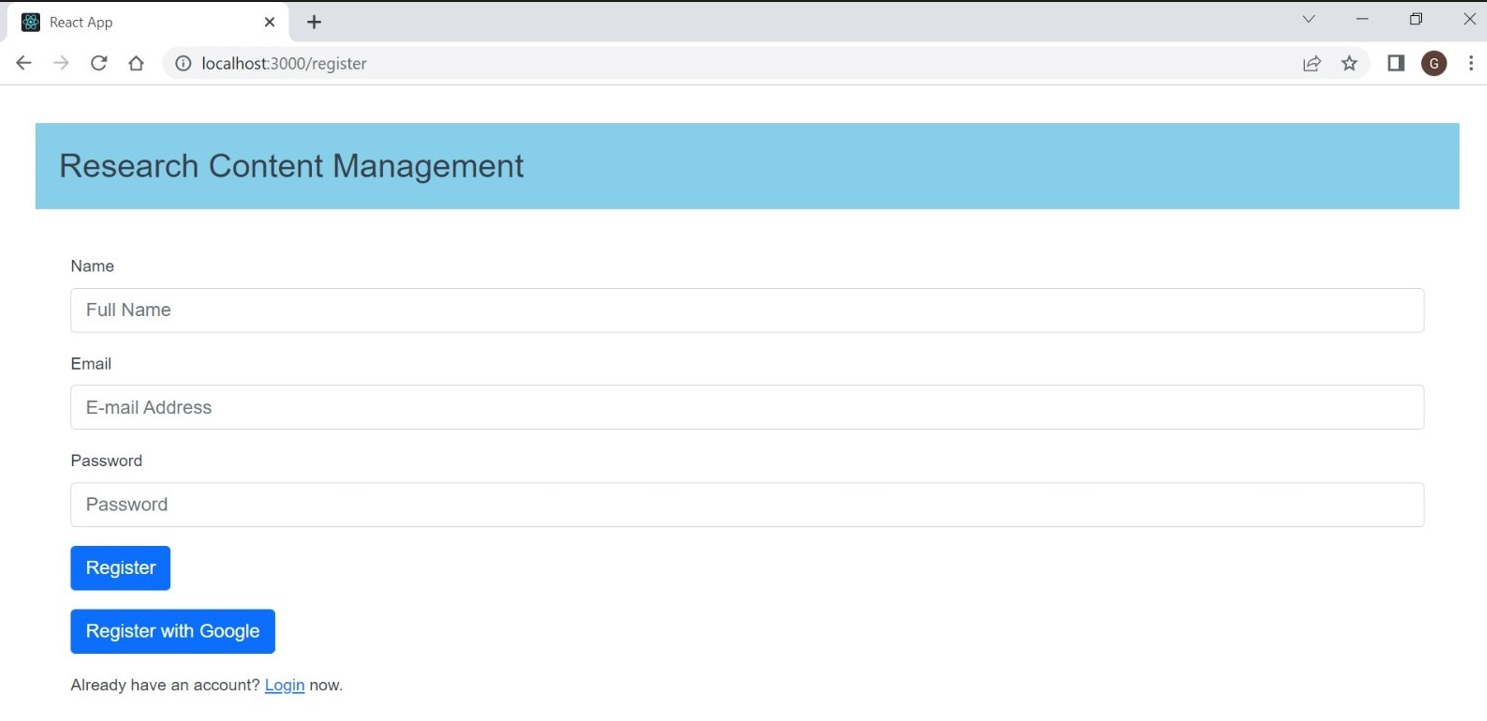
\includegraphics[width=11cm,height=6cm]{./images/register.png}
	\vspace{-0.5cm}
	\caption{Register Page}
	\label{fig:register}
\end{figure}

\paragraph{\textbf{Login:}} For existing users, we have develop a login component shown in Figure \ref{fig:login}.
\begin{figure}[htbp]
	\centering
	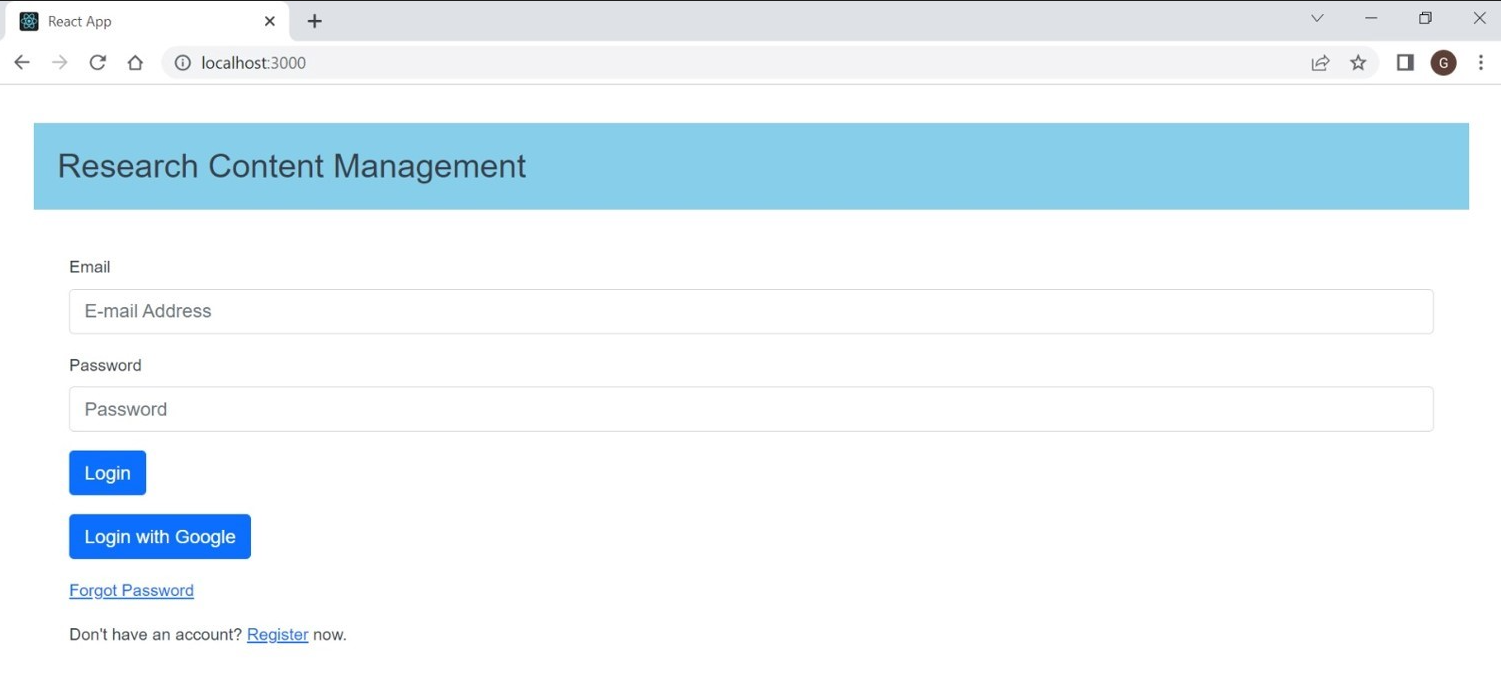
\includegraphics[width=11cm,height=5cm]{./images/login.png}
	\vspace{-0.5cm}
	\caption{Login Page}
	\label{fig:login}
\end{figure}
 Once a user has successfully created/registered an account he/she can login to website using his/her email address and password.
 Alternatively, the user can also login with Google account as we have the option of registering using Google account. If the user forget his/her password, the user can reset the password via  forgot password link, which we provide on the login page. Upon clicking the link, the user has to enter his registered email address in order to reset the password. 

\paragraph{\textbf{Dashboard:}} We have developed a dashboard component for the users to upload, search and view papers upon login. The dashboard consists of website name to the left and the user can see his name, email address and logout button to the right. This dashboard gives the user a quick glance of user details.

\paragraph{\textbf{Upload:}} We have developed an upload component for the users to upload their interested papers shown in Figure \ref{fig:upload}.This page allows a user to upload a research paper on which he/she is currently working or previous research papers which he/she worked on. For making the uploaded paper unique, there are several factors taken into consideration. The paper which user wants to upload should be of pdf format, should choose a topic for the paper, year of publishing for the paper, title of the paper, and finally technique of the paper. By choosing the above metrics, each paper represents unique. When the user clicks on submit button given in Figure \ref{fig:upload}, the paper is directly uploaded to the Firebase server which later can be accessed.
\begin{figure}[h]
	\centering
	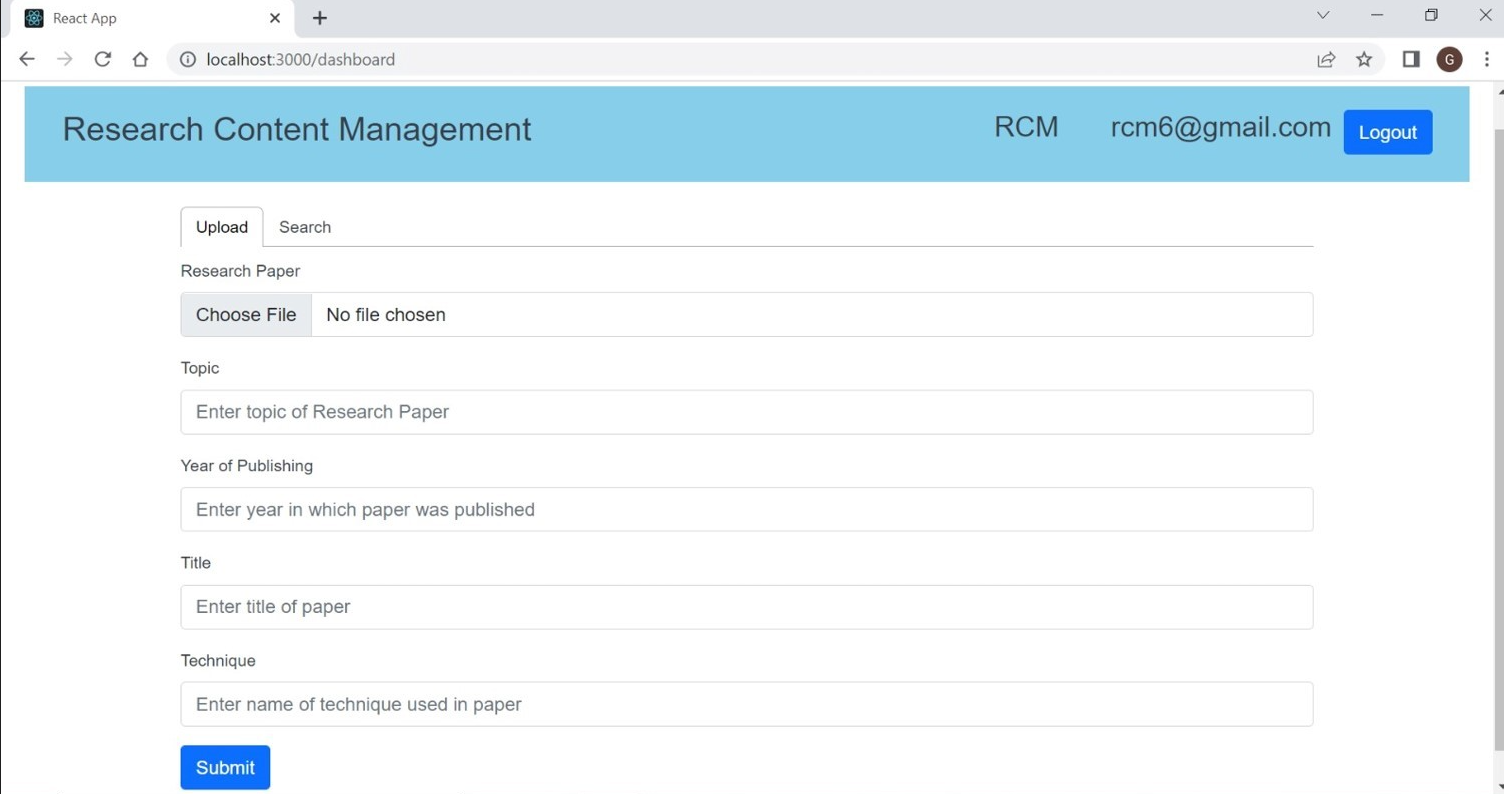
\includegraphics[width=11cm,height=6cm]{./images/upload.png}
	\vspace{-0.5cm}
	\caption{Upload Page}
	\label{fig:upload}
\end{figure}

\paragraph{\textbf{Search:}} Upon login, a user can search interested papers that have been already uploaded by him/her. For this, we have developed a search component. It uses the Firebase database finding papers based on topic, title, year or technique. Upon entering these key values, the user has to enter the search button shown in Figure \ref{fig:search}. Upon clicking on search button, the component interacts with the Firebase database and find all matching papers stored in the Firebase database. For this, we have implemented effective 
search technique.
\begin{figure}[h]
	\centering
	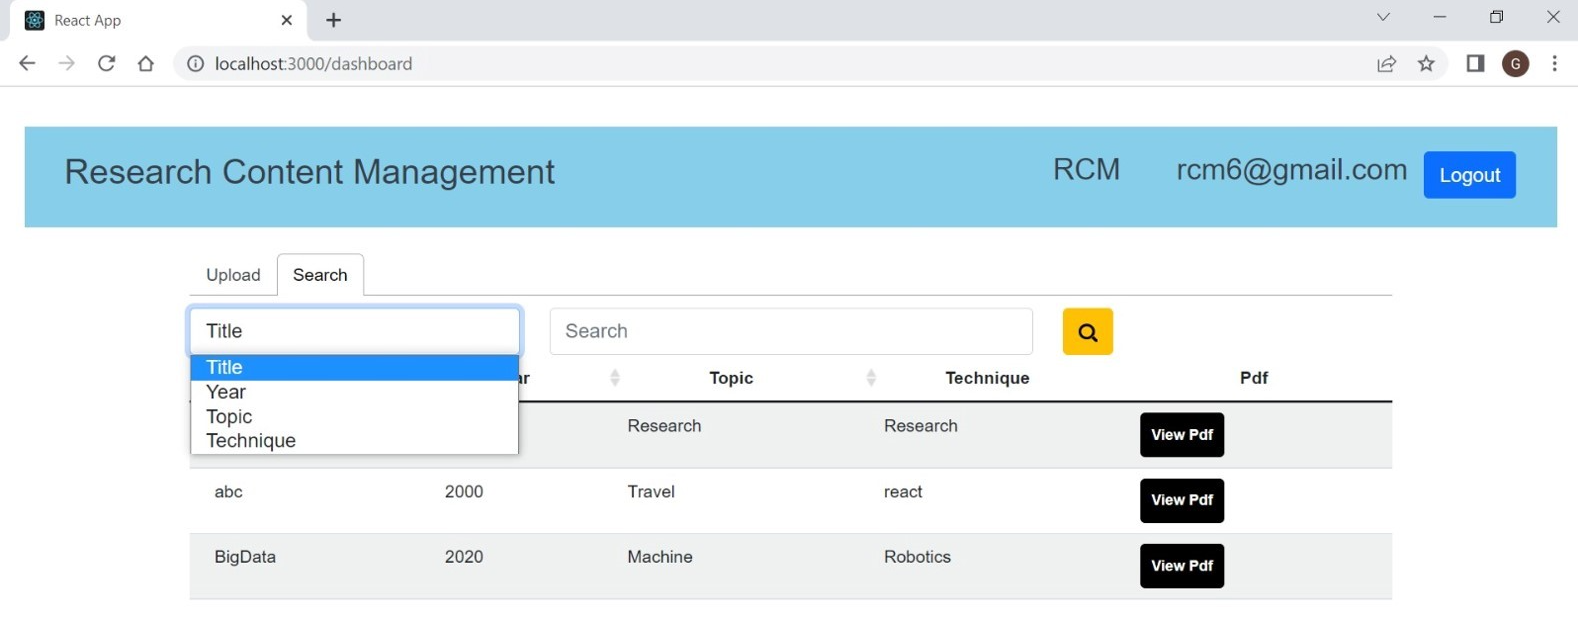
\includegraphics[width=11cm,height=6cm]{./images/search.png}
	\vspace{-0.5cm}
	\caption{Search Page}
	\label{fig:search}
\end{figure}

\paragraph{\textbf{View:}} Upon searching papers, the user may wish to view/read a specific paper. For this, we have developed view component shown in Figure \ref{fig:view}. After search operation, there is a view button on each matched paper. When the user clicks on a specific paper, view component will help the user to read/view the paper along with comments facility. If the user wants to add comments for the paper, he/she needs to enter the note in comments box and to click on post comment button. Then, the comment for the paper will be stored in database with timestamp. When user clicks on show comments button, the comments which are posted for the paper is displayed as list with the timestamp.
\begin{figure}[h]
	\centering
	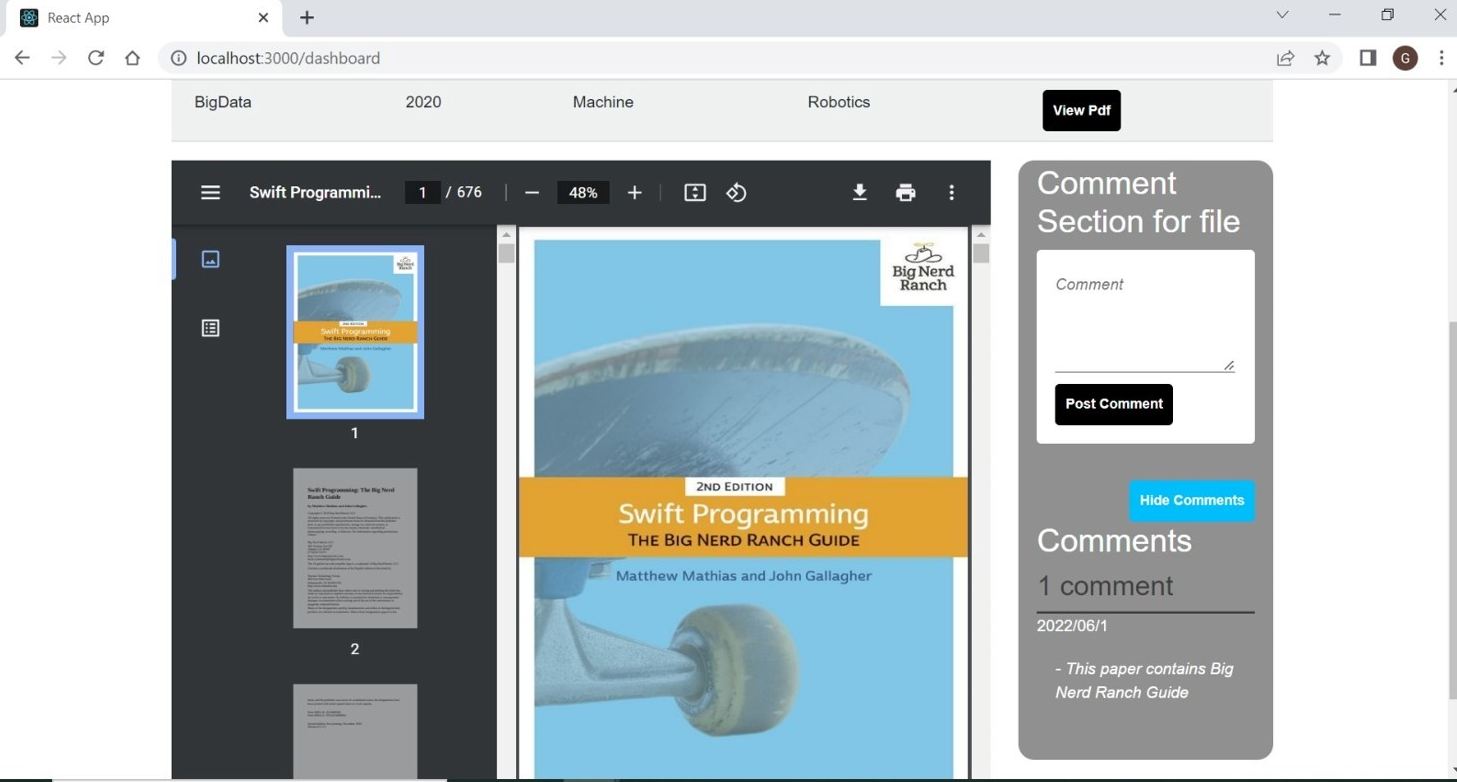
\includegraphics[width=11cm,height=6cm]{./images/view.png}
	\vspace{-0.5cm}
	\caption{Search Page}
	\label{fig:view}
\end{figure}





